%% LyX 2.1.1 created this file.  For more info, see http://www.lyx.org/.
%% Do not edit unless you really know what you are doing.
\documentclass[12pt,english]{article}
\usepackage[T1]{fontenc}
\usepackage[latin9]{inputenc}
\usepackage[a4paper]{geometry}
\geometry{verbose,tmargin=1.25cm,bmargin=1.25cm,lmargin=1.25cm,rmargin=1.25cm,headheight=1.25cm,headsep=1.25cm,footskip=1.25cm}
\usepackage{graphicx}
\usepackage{babel}
\begin{document}

\title{Week 5: Quarter Wave Transformer\\
with FDTD in 1D Systems}


\author{Sankeerth.D\\
EE13B102\\
Electrical Engineering}
\maketitle
\begin{abstract}
Transmittance can be increased by introducing a qwarter wave plate
inbetween the slab and air. Impedance matching, ideally, wil make
all the light pass through, reducing back reflection.
\end{abstract}

\section{Introduction}

Again, the normallized equation is solved here, and the units and
differential increments are adjusted to fit the problem parameters.
QWT's have their refractive index as the geometric mean of the product
of the refractive indices of the adjascent media. Here, two of these
are used on either side of the slab.


\section{Selection of Units}

Where H1 and E1 are the scaled E and H. Scale the units of x and t
to obtain equations identical to the ones shown above. for the frequency
of 2.4 GHz, In the middle layer, it turns out that the ripples are
too high for a time step of 0.333e-10 seconds. So, for this case,
It's conveniant to choose t to be in multiples of 0.1666e-10, and
x to be in multiples of 0.5e-2 metres. Then, the update equations
will be identical to the normallized case.

1 foot occupies 30 centimeter, so 60 units of x should do. The length
of the quarter wave plate is 1.68 centimeter. 3 units of x, which
is 1.5 centimeter, is used here. Frequency of 2.4 GHz is obtained
using a sinusoidal source, and source is on for 3 cycles. This creates
a frequency spread, roughly between 2.2 and 2.6 GHz. The source spectrum
is as shown an follows:

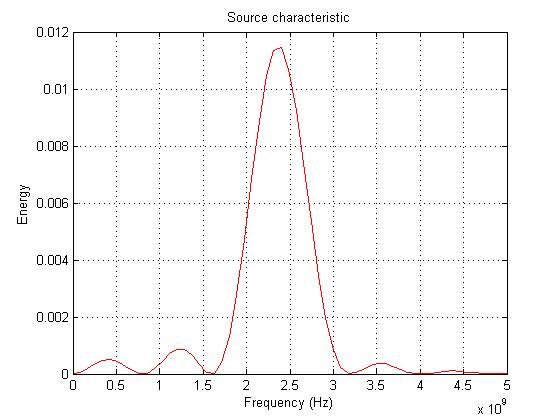
\includegraphics[width=0.5\linewidth]{source}

The total length is 300 units, which is 150 centimeter. To record
only one time reflection, and provent multiple reflections, the slab
is placed at 2{*}xdim/3 from the source.


\section{Observation}

On runnning the ssimulation for 700 time units, which is 11.66 nanoseconds,
a single reflection and transmission can be captured.

Before introducong the QWT, the reflectance and transmittance are
as follows (for epsilon =12, mu = 1):

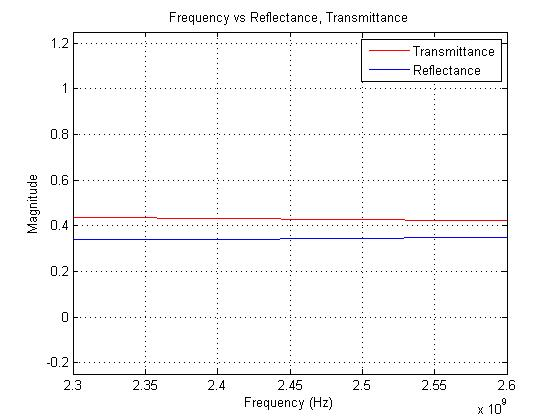
\includegraphics[width=0.45\linewidth]{withoutQWT} 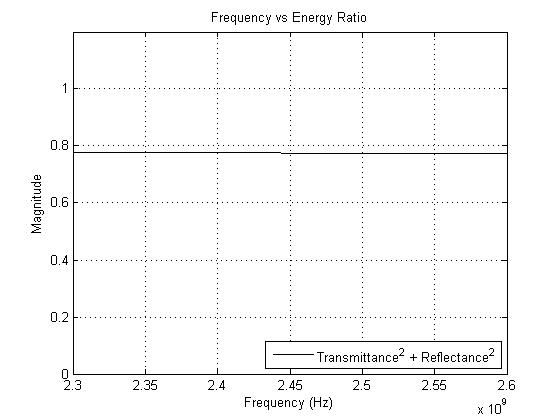
\includegraphics[width=0.45\linewidth]{withoutQWTsource}

A large portion of the wave got reflected back in this case. Observe
that less than 80 percent of the total energy is reflected+transmitted
in the first reflection. Also, as expected, as the permittivities
are independant of frequency, the characteristics are also independant
of frequency (around 2.4 GHz.). Since the medium is nonmagnetic (unlike
in the previous case where there's mu = 2) Fresnel's equations can
be applied.
\[
Reflectance=\frac{(n-1)^{2}}{(n+1)^{2}}
\]


where n = sqrt(12). Plugging this in, we get reflectance = 0.305,
close to whar we get in simulation.

On placing a dielectric across the 1 foot slab, there would be a somewhat
slower transition between the media and it is reasonable to expect
a higher transmittance. Also, since the QWT is designed such that
reflective component destructively interferes across the quarter wave,
reflectance reduces sharply, as can be seen below:

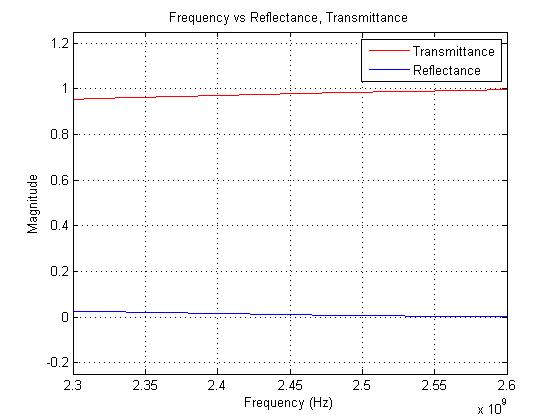
\includegraphics[width=0.45\linewidth]{withQWT} 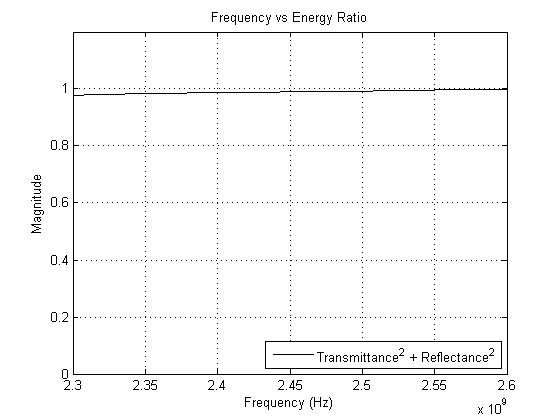
\includegraphics[width=0.45\linewidth]{withQWTsource}

One can clearly see thet these lines aren't horizontal. This is because
we are measuring the interfered portion of wave (across the QWT).
Since there's a frequency spread, and we have used a 1.5 centimeter
QWT, the ideal transmission happens at 2.6 GHz. If we were to use
a more accurate 1.68 cm, we would've gotten the peak at 2.4 GHz, but
this is good enough for a demonstration. As expected, most of the
light passes through.


\section{Result and Discussion}

Note that this probem can be solved using the same update equations
and different spacing $\Delta x$ and $\Delta t$. The discretization
chosen here is such that in the high refractive index material, the
gaussian pulse is not very sharp. If it were to be sharp, Due to courant
factor, the inaccuracy and error in simulation increases by multiplee
folds, and numerous ripples can be seen in the medium.

As one can see, The medium is not frequency selective, and The reason
for the very small slope in the second case is because what we measure
is the interfered light, the sum of it's reflected components across
1.68 centimeter. Since defferent frequencies have different powers
after this interference, we see this frequency dependnce.
\end{document}
